\documentclass[11pt]{article}
\usepackage[margin=1in]{geometry}
\usepackage{amsmath,amssymb,amsthm,bm}
\usepackage{graphicx,booktabs}
\usepackage[hidelinks]{hyperref}

\newtheorem{proposition}{Proposition}
\newtheorem{lemma}[proposition]{Lemma}
\newtheorem{theorem}[proposition]{Theorem}
\newtheorem{corollary}[proposition]{Corollary}
\theoremstyle{remark}
\newtheorem{remark}[proposition]{Remark}

\newcommand{\R}{\mathbb{R}}
\newcommand{\1}{\mathbf{1}}
\newcommand{\s}{\mathbf{s}}
\newcommand{\y}{\mathbf{y}}
\newcommand{\vv}{\mathbf{v}}
\newcommand{\m}{\mathbf{m}}
\newcommand{\M}{\mathbf{M}}
\newcommand{\Sm}{\mathbf{S}}
\newcommand{\Y}{\mathbf{Y}}
\newcommand{\aff}{\operatorname{aff}}
\newcommand{\conv}{\operatorname{conv}}
\newcommand{\relint}{\operatorname{relint}}

\title{Which precinct normalizations preserve the linear mixing model?}
\author{Notes for \texttt{voting-unmixing-ph}}
\date{2026-11-09}

\begin{document}
\maketitle

\begin{abstract}
Comparing 2013/2016 (row-max normalization) with 2019--2025 (per-ballot
normalization) on real returns mixes two effects: the normalization and a large
change in the political landscape. This note isolates the first one with a proof
and noise-free and noisy toy data. Dividing by the number of ballots keeps the
linear mixing model (LMM) exact, with abundances equal to voter fractions.
Dividing by the vote sum keeps it exact, but the abundances become vote shares
and ballot width is lost. Dividing by the row maximum breaks the sum-to-one LMM
whenever the mixed voter types disagree on their top candidate: precincts lie
\emph{outside} the simplex of the normalized pure types. No choice of $p$
endmembers fits them exactly. On toy data this inflates MVSA's endmembers and
gives them negative loadings that the true types do not have. Figures and the
table come from \texttt{make\_figures.py} (seeded, synthetic, no election data
needed). Notation follows Li and Bioucas-Dias (2008), the MVSA paper.
\end{abstract}

\section{Setup}

\paragraph{Notation.} Candidates are indexed by $\ell=1,\dots,L$, voter types
(endmembers) by $i=1,\dots,p$, and precincts (pixels) by $j=1,\dots,n$. As in
the MVSA paper, the LMM is
\begin{equation}
  \Y = \M\Sm \quad\text{s.t.}\quad \Sm\succeq 0,\ \ \1_p^\top\Sm = \1_n^\top,
  \label{eq:lmm}
\end{equation}
with data $\Y=[\y_1,\dots,\y_n]$, mixing matrix $\M=[\m_1,\dots,\m_p]$ and
abundance matrix $\Sm=[\s_1,\dots,\s_n]$. Entry $[\Sm]_{ij}$ is the fraction of
endmember $i$ in precinct $j$, so each column $\s_j$ lies in the probability
simplex $\Delta_p := \{\s\in\R^p : \s\succeq 0,\ \1_p^\top\s = 1\}$. The MVSA
paper writes \eqref{eq:lmm} in the $p$-dimensional signal subspace, where $\M$
is square and $\mathbf Q\equiv\M^{-1}$. We stay in $\R^L$ ($\M$ is $L\times p$).
The constraints are the same. Estimates carry hats: $\hat\M$, $\hat\Sm$.

\paragraph{Generative model.} Precinct $j$ has $B_j$ ballots. A voter of type $i$
marks candidate $\ell$ with probability $[\M]_{\ell i}\in[0,1]$, and
$[\Sm]_{ij}$ is the fraction of precinct $j$'s voters of type $i$. Each type has
an expected number of names per ballot $c_i := \1_L^\top\m_i$; write
$\mathbf c = [c_1,\dots,c_p]^\top$. The expected vote matrix
$\mathbf V=[\vv_1,\dots,\vv_n]$ has columns
\begin{equation}
  \underbrace{\vv_j}_{\text{vote}} = \underbrace{B_j}_{\text{ballot}}\ \underbrace{\M}_{\text{vote/ballot}}\ \underbrace{\s_j}_{\text{ballot/ballot}} .
  \label{eq:counts}
\end{equation}

\paragraph{Units.} Two things are counted: a \emph{ballot} (one voter, who casts
one ballot) and a \emph{vote} (one name marked on one ballot). A \emph{top vote}
is a vote for the precinct's top candidate $\ell^\ast=\arg\max_\ell[\vv_j]_\ell$.
Units are written under braces or in upright brackets, e.g.\ [vote/ballot]. A
bracket with a subscript, like $[\M]_{\ell i}$, is still a matrix entry.
Unit symbols are singular, as in SI ([m/s], [mol/mol]): in [vote/vote] both
sides are the same unit, the vote. Each short unit abbreviates a ratio of two totals over
precinct $j$ (or over one type's voters). The finest data are clustered-precinct
totals, so [vote/ballot] is a precinct average, never a count on one physical
ballot. The denominator is always an observed count: all ballots cast $B_j$, all
votes cast $\1_L^\top\vv_j$ (marks summed over every candidate and ballot), or
the top candidate's votes. Numerators split by type are latent. Spelled out:
\begin{center}
\small
\begin{tabular}{lll}
\toprule
unit & spelled out & where \\
\midrule
vote/ballot & votes for $\ell$ / all ballots cast in $j$ & per-ballot $\y_j$ \\
ballot/ballot & type-$i$ ballots / all ballots cast in $j$ (voter fraction) & per-ballot abundance \\
vote/vote & votes for $\ell$ / all votes cast in $j$ & vote-sum $\y_j$ \\
vote/vote & type-$i$ votes / all votes cast in $j$ (vote share) & vote-sum abundance \\
vote/top vote & votes for $\ell$ / votes for $\ell^\ast$ in $j$ & row-max $\y_j$ \\
\bottomrule
\end{tabular}
\end{center}
For a type's profile the denominator is that type's ballots: $[\M]_{\ell i}$ is
[type-$i$ votes for $\ell$ / type-$i$ ballots] and $c_i$ is [type-$i$ votes /
type-$i$ ballots]. Same-kind ratios are dimensionless; the unit records which
whole they are a fraction of, which matters (see \emph{Units check}).
\begin{center}
\small
\begin{tabular}{lll}
\toprule
symbol & meaning & units \\
\midrule
$B_j$ & ballots cast in precinct $j$ & ballot \\
$[\vv_j]_\ell$ & votes for candidate $\ell$ in precinct $j$ & vote \\
$[\M]_{\ell i}$ & chance a type-$i$ ballot marks $\ell$ & type-$i$ votes for $\ell$ / type-$i$ ballots \\
$[\Sm]_{ij}$ & voter fraction of type $i$ in precinct $j$ & type-$i$ ballots / all ballots in $j$ \\
$c_i$ & names per type-$i$ ballot & type-$i$ votes / type-$i$ ballots \\
\bottomrule
\end{tabular}
\end{center}

Sampling noise is set aside until Section~\ref{sec:toy}. Everything below holds
for the expectation, i.e.\ in the limit of large $B_j$.

The abundance sum-to-one constraint (ASC) $\1_p^\top\Sm = \1_n^\top$ is what
matters below. MVSA imposes it ($\1_p^\top\mathbf Q\Y = \1_n^\top$), and so does
SUNSAL with \texttt{addone="yes"}. If the ASC is dropped, $\Y=\M\Sm$ with
$\Sm\succeq 0$ alone is a cone model.

\paragraph{Normalizations.} Three are in use or under consideration:
\begin{align*}
  \text{per-ballot:}&\quad \y_j = \vv_j / B_j &&\text{[vote/ballot]}, \\
  \text{vote-sum:}&\quad \y_j = \vv_j / \1_L^\top\vv_j &&\text{[vote/vote]}, \\
  \text{row-max:}&\quad \y_j = \vv_j / \textstyle\max_\ell\, [\vv_j]_\ell &&\text{[vote/top vote]}.
\end{align*}
The last two have the form $\y = \vv/d(\vv)$, with $d$ positively homogeneous of
degree one, $d(\alpha\vv)=\alpha\,d(\vv)$ for $\alpha>0$. Then $B_j$ cancels:
$\y_j = \M\s_j / d(\M\s_j)$.

In the single-precinct statements below we drop the index $j$: $\s\in\Delta_p$
is one column of $\Sm$, with entries $s_i := [\Sm]_{ij}$.

Table~\ref{tab:units} puts the units of every quantity side by side.
\begin{table}[ht]
\centering
\small
\resizebox{\linewidth}{!}{%
\begin{tabular}{llllll}
\toprule
 & $\y_j$ & normalized type $\tilde\m_i$ & abundance $=$ share of \dots & width $\1_L^\top\y_j$ & $\Lambda$ \\
\midrule
per-ballot & vote/ballot & $\m_i$ \ [vote/ballot] & ballots (voter fraction) & names per ballot [vote/ballot] & --- \\
vote-sum & vote/vote & $\m_i/c_i$ \ [vote/vote] & votes (vote share) & $1$ [vote/vote] & $1$ \\
row-max & vote/top vote & $\m_i/\max_\ell[\M]_{\ell i}$ \ [vote/own-top vote] & none: weights sum to $\Lambda$ & vote/top vote & $\ge 1$ \\
\bottomrule
\end{tabular}}
\caption{Units of each quantity under each normalization.}
\label{tab:units}
\end{table}

\paragraph{Units check.} In ordinary dimensional analysis the vote-sum and
row-max ratios are both dimensionless (vote/vote). What the denominator counts
still matters, because the LMM is a weighted average: $\y_j=\sum_i[\Sm]_{ij}\m_i$
only adds up if each abundance is a share of the denominator's quantity, and that
quantity is split exactly among the types. Every ballot belongs to exactly one
type, so ballot shares sum to one. Every vote is cast by exactly one type, so
vote shares sum to one. Top votes are not split this way. Each type's profile is
divided by its \emph{own} top candidate $\ell(i)$, while the precinct is divided
by the precinct's top candidate $\ell^\ast$. Proposition~\ref{prop:rowmax} makes
this exact.

\section{Results}

\begin{proposition}[per-ballot]\label{prop:ballot}
\[
  \underbrace{\y_j}_{\text{vote/ballot}} = \underbrace{\M}_{\text{vote/ballot}}\ \underbrace{\s_j}_{\text{ballot/ballot}},
  \qquad
  \underbrace{\1_L^\top\y_j}_{\text{vote/ballot}} = \underbrace{\mathbf c^\top}_{\text{vote/ballot}}\ \underbrace{\s_j}_{\text{ballot/ballot}},
\]
i.e.\ $\Y=\M\Sm$. The LMM \eqref{eq:lmm} holds exactly with the true mixing
matrix and with abundances equal to the voter fractions. The width is the mean
number of names per ballot.
\end{proposition}
\begin{proof}
Divide \eqref{eq:counts} by $B_j$.
\end{proof}

\begin{remark}[blank and overvoted ballots]\label{rem:blank}
A ballot that leaves the senate race blank, or overvotes it (all its senate marks
are voided), adds nothing to $\vv_j$ but is counted in $B_j$. This is a type with
$\m_0=\mathbf{0}$, so Proposition~\ref{prop:ballot} still holds with $p+1$ types,
one at the origin. Such ballots lower the width. If instead the denominator
excludes them, $\y_j = \sum_{i\ge 1}\frac{s_{i}}{1-s_{0}}\m_i$, which is still an
LMM, over voters who cast a counted senate ballot. What matters is that the
denominator \emph{counts voters} and does not depend on how they voted. A
denominator $r_jB_j$ with a precinct-varying factor $r_j$ [counted
ballots / ballots cast] gives $\1_p^\top\hat\s_j = 1/r_j$, which violates the ASC:
the abundances are then shares of a quantity that the types do not split
exactly. The 2025
\texttt{numberOfValidBallot} column is such a case: $r_j$ has median $1.08$
and differs by region.
\end{remark}

\begin{lemma}[homogeneous normalizations]\label{lem:homog}
Let $d$ be positively homogeneous with $d(\m_i)>0$. Write
$\tilde\m_i := \m_i/d(\m_i)$ for the normalized pure types and
$\tilde\M = [\tilde\m_1,\dots,\tilde\m_p]$. Then
\begin{equation}
  \y = \sum_{i=1}^p w_i(\s)\,\tilde\m_i,\qquad
  w_i(\s) = \frac{s_i\, d(\m_i)}{d(\M\s)} \ge 0,\qquad
  \sum_i w_i(\s) = \Lambda(\s) := \frac{\sum_i s_i\, d(\m_i)}{d\!\left(\sum_i s_i\m_i\right)} .
  \label{eq:lambda}
\end{equation}
\end{lemma}
\begin{proof}
$\y = \M\s/d(\M\s) = \sum_i s_i\m_i/d(\M\s) = \sum_i \frac{s_i d(\m_i)}{d(\M\s)}\,\tilde\m_i$.
\end{proof}

Units: $s_i$ is [ballot/ballot], and $d(\m_i)$ and $d(\M\s)$ are both
``$d$-quantity per ballot''. So $w_i$ is the fraction of the precinct's
$d$-quantity that type $i$ contributes, \emph{where type $i$'s contribution is
measured with its own $d$}.

So $\y$ lies in the cone of the $\tilde\m_i$ in every case. It lies in their
\emph{simplex} (the LMM \eqref{eq:lmm} with mixing matrix $\tilde\M$) exactly when
$\Lambda(\s)=1$.

\begin{proposition}[vote-sum]\label{prop:sum}
For $d(\vv)=\1_L^\top\vv$, $\Lambda\equiv 1$. The LMM holds exactly with mixing
matrix $\tilde\M$, $\tilde\m_i = \m_i/c_i$, and abundances
\[
  \underbrace{[\hat\Sm]_{ij}}_{\text{vote/vote}} = \frac{\overbrace{c_i}^{\text{vote/ballot}}\ \overbrace{[\Sm]_{ij}}^{\text{ballot/ballot}}}{\underbrace{\mathbf{c}^\top\s_j}_{\text{vote/ballot}}},
  \qquad
  \underbrace{\tilde\m_i}_{\text{vote/vote}} = \frac{\overbrace{\m_i}^{\text{vote/ballot}}}{\underbrace{c_i}_{\text{vote/ballot}}},
\]
the share of precinct $j$'s \emph{votes} cast by type $i$. The map
$\s_j\mapsto\hat\s_j$ is a bijection of $\Delta_p$ (inverse
$[\Sm]_{ij}\propto[\hat\Sm]_{ij}/c_i$), but it depends on $\mathbf{c}$, which
cannot be identified from the data: every $\y_j$ and every $\tilde\m_i$ sums to
one. Voter fractions and ballot width are therefore both lost.
\end{proposition}
\begin{proof}
$d$ is linear, so $d(\sum_i s_i\m_i)=\sum_i s_i d(\m_i)$ and $\Lambda=1$ in
\eqref{eq:lambda}. Rescaling any $\m_i$ leaves $\tilde\m_i$, and hence all data,
unchanged, so $\mathbf{c}$ is not identifiable.
\end{proof}

\begin{proposition}[row-max lies outside the simplex]\label{prop:rowmax}
Let $d(\vv)=\max_\ell [\vv]_\ell$ and write $\tilde\M$ for the
row-max-normalized types. Then $\Lambda(\s)\ge 1$, so
\[
  \y = \Lambda(\s)\,\bar\y,\qquad \bar\y := \sum_i \frac{w_i(\s)}{\Lambda(\s)}\tilde\m_i \in \conv(\tilde\m_1,\dots,\tilde\m_p).
\]
The precinct sits on the ray through a point of the simplex of the normalized
pure types, a factor $\Lambda\ge 1$ beyond it. Equality $\Lambda(\s)=1$ holds iff
some candidate $\ell$ is a top candidate of every type present in the precinct,
i.e.\ $[\M]_{\ell i}=\max_{\ell'} [\M]_{\ell' i}$ for all $i$ with $s_i>0$.
\end{proposition}
\begin{proof}
Let $\ell^\ast$ be a maximizing index of $\M\s$. Then
\[
  d(\M\s) = \sum_i s_i [\M]_{\ell^\ast i} \le \sum_i s_i \max_{\ell'} [\M]_{\ell' i} = \sum_i s_i\, d(\m_i),
\]
so $\Lambda\ge1$. Since $s_i\ge 0$, equality holds iff
$[\M]_{\ell^\ast i}=\max_{\ell'}[\M]_{\ell' i}$ for every $i$ with $s_i>0$. If some
$\ell$ tops every type present, then $[\M\s]_\ell=\sum_i s_i d(\m_i)$, which is
the largest any entry of $\M\s$ can be. So $\ell$ is a maximizer and equality
holds. This gives the ``iff''.
\end{proof}

\paragraph{Units reading of the proof.} Multiply the numerator and denominator
of $w_i$ by $B_j$:
\[
  w_i = \frac{\overbrace{s_iB_j}^{\text{type-$i$ ballots}}\ \overbrace{d(\m_i)}^{\text{type-$i$ votes for $\ell(i)$ / type-$i$ ballots}}}{\underbrace{B_j\,d(\M\s)}_{\text{votes for $\ell^\ast$}}}
  = \frac{\text{type-$i$ votes for its own top candidate $\ell(i)$}}{\text{all votes for the precinct's top candidate $\ell^\ast$}},
\]
\[
  \Lambda = \sum_i w_i = \frac{\sum_i(\text{type-$i$ votes for $\ell(i)$})}{\sum_i(\text{type-$i$ votes for $\ell^\ast$})} \ \ge\ 1,
\]
because each type votes for its own top candidate at least as often as for
$\ell^\ast$. The units match (vote/vote), but the numerator counts votes for
different candidates for different types. For vote-sum the numerator would be
type-$i$ votes for \emph{anyone}, which do partition the denominator, so
$\Lambda=1$.

\begin{remark}[row-max as a stand-in for the voter count]\label{rem:proxy}
Row-max is tempting when there is no ballot count, because its denominator grows
with turnout:
\[
  \underbrace{\max_\ell[\vv_j]_\ell}_{\text{top vote}} = \underbrace{B_j}_{\text{ballot}}\ \underbrace{f_j}_{\text{top vote/ballot}},
  \qquad f_j := \max_\ell[\M\s_j]_\ell,
\]
where $f_j$ is the top candidate's share of ballots. Replacing $B_j$ by $B_jf_j$
works only in two steps, each with its own condition.
\begin{enumerate}
  \item \emph{Exact LMM: one candidate $\ell_0$ tops every voter type}, and
  therefore every precinct. This is the $\Lambda=1$ case of
  Proposition~\ref{prop:rowmax}. The denominator is then
  $[\vv_j]_{\ell_0}=\mathbf e_{\ell_0}^\top\vv_j$, a \emph{linear} function of the
  votes. The proof of Proposition~\ref{prop:sum} with $d=\mathbf e_{\ell_0}^\top$
  gives an exact LMM with abundances
  \[
    \underbrace{[\hat\Sm]_{ij}}_{\text{top vote/top vote}} = \frac{[\Sm]_{ij}\,[\M]_{\ell_0 i}}{[\M\s_j]_{\ell_0}},
  \]
  type $i$'s share of $\ell_0$'s votes, not of the voters.
  \item \emph{Voter fractions: $f_j$ is also the same in every precinct.} This
  needs every type to mark $\ell_0$ at the same rate, $[\M]_{\ell_0 i}=f$ for all
  $i$, i.e.\ a candidate on essentially every ballot. Then the denominator is
  $fB_j$, and Proposition~\ref{prop:ballot} holds up to the constant $f$.
\end{enumerate}
Agreement within each precinct is not enough. If the top candidate differs
between precincts, each precinct is divided by a different linear function, and
the normalized types $\tilde\m_i$ change from precinct to precinct.

In the returns, neither condition holds (Table~\ref{tab:proxy}; computed in
notebook~13, ``Is row-max a stand-in for the voter count?''). Without a ballot
count, a denominator that is linear in the votes and the same for every precinct,
such as vote-sum (Proposition~\ref{prop:sum}), needs neither condition. The cost
is that abundances become vote shares rather than voter fractions.
\end{remark}

\begin{table}[ht]
\centering
\small
\resizebox{\linewidth}{!}{%
\begin{tabular}{lllll}
\toprule
 & precincts topped by national \#1 & different top candidates & $f_j$, median (IQR) & corr(row-max denom., voters) \\
\midrule
2013 & 46\% (Poe) & 18 & --- & --- \\
2016 & 13\% (Villanueva); Sotto tops 20\% & 26 & --- & --- \\
2019 & 42\% (Villar) & 30 & 0.60 (0.53--0.66) & 0.83 \\
2022 & 42\% (Padilla) & 32 & 0.54 (0.48--0.60) & 0.76 \\
2025 & 40\% (Go); Aquino tops 35\% & 33 & 0.54 (0.46--0.64) & 0.75 \\
\bottomrule
\end{tabular}}
\caption{Is row-max a stand-in for the voter count? Senatorial returns at the
sweep's preprocessing settings. 2013 and 2016 have no voter count, so $f_j$ and
the correlation cannot be computed.}
\label{tab:proxy}
\end{table}

Proposition~\ref{prop:rowmax} shows that the \emph{true} types do not give a
simplex fit. The next result rules out \emph{any} $p$ endmembers. This matters
because MVSA is free to choose its own.

\begin{theorem}[row-max admits no exact $p$-endmember LMM]\label{thm:rowmax}
Assume (i) $\M$ has full column rank $p\ge 2$; (ii) each type has a unique top
candidate $\ell(i)=\arg\max_{\ell} [\M]_{\ell i}$; and (iii) at least two types
differ in their top candidate, $\ell(i_1)\ne \ell(i_2)$. Let
$\mathcal Y = \{\M\s/\max_\ell[\M\s]_\ell : \s\in\Delta_p\}$ be the set of
row-max-normalized precincts. Then $\mathcal Y$ is not contained in any affine
subspace of dimension $p-1$. Hence there are no $\hat\M\in\R^{L\times p}$ and
$\hat\s(\s)\in\Delta_p$ with $\y(\s)=\hat\M\hat\s(\s)$ for all $\s$. The same
holds for any set of precincts whose columns $\s_j$ are dense in an open subset of
$\Delta_p$ that meets both regions $R_{\ell(i_1)}$ and $R_{\ell(i_2)}$ defined
below.
\end{theorem}
\begin{proof}
For a candidate $\ell$, let
$R_\ell=\{\s\in\relint\Delta_p : [\M\s]_\ell > [\M\s]_{\ell'}\ \forall \ell'\ne \ell\}$.
It is relatively open, by continuity. By (ii), the vertex $\mathbf e_{i_1}$ has the
strict maximizer $\ell(i_1)$, so points of $\relint\Delta_p$ near $\mathbf e_{i_1}$
lie in $R_{\ell(i_1)}$, which is therefore nonempty. Likewise
$R_{\ell(i_2)}\neq\emptyset$.

On $R_\ell$, $\y(\s)=\M\s/(\mathbf e_\ell^\top\M\s)$ is smooth. Its differential
along a tangent direction $\bm\delta$ ($\1_p^\top\bm\delta=0$) is
$D\y\,\bm\delta = (\mathbf I-\y\,\mathbf e_\ell^\top)\M\bm\delta/(\mathbf e_\ell^\top\M\s)$.
If this vanishes, $\M\bm\delta = \alpha\M\s$ with
$\alpha=\mathbf e_\ell^\top\M\bm\delta/\mathbf e_\ell^\top\M\s$. Then
$\bm\delta=\alpha\s$ by (i), and $0=\1_p^\top\bm\delta=\alpha$, so
$\bm\delta=\mathbf 0$. The differential is injective, so $\y(R_\ell)$ contains a
$(p-1)$-dimensional embedded piece and $\dim\aff\,\y(R_\ell)=p-1$. Every point of
$\y(R_\ell)$ has $y_\ell=1$, so $\aff\,\y(R_\ell)\subseteq\{y_\ell=1\}$.

Write $\ell_1=\ell(i_1)$ and $\ell_2=\ell(i_2)$. Suppose
$\mathcal Y\subseteq\mathcal A$ with $\mathcal A$ affine and
$\dim\mathcal A=p-1$. Then $\aff\,\y(R_{\ell_1})\subseteq\mathcal A$, and the
dimensions are equal, so
$\mathcal A=\aff\,\y(R_{\ell_1})\subseteq\{y_{\ell_1}=1\}$. In the same way
$\mathcal A\subseteq\{y_{\ell_2}=1\}$. But for $\s\in R_{\ell_1}$,
$y_{\ell_2}(\s)=[\M\s]_{\ell_2}/[\M\s]_{\ell_1}<1$. This is a contradiction.
Finally, any $\{\hat\M\hat\s:\hat\s\in\Delta_p\}$ lies in $\aff(\hat\m_1,\dots,\hat\m_p)$,
which has dimension at most $p-1$. The dense-subset version follows because the
argument only uses open pieces of $R_{\ell_1}$ and $R_{\ell_2}$.
\end{proof}

\begin{corollary}[what row-max preserves]\label{cor:cone}
Under row-max the cone model is still exact: $\y=\tilde\M\mathbf w$ with
$\mathbf w\succeq 0$ and $\1_p^\top\mathbf w=\Lambda(\s)\ge 1$. The failure comes
from the ASC, which both MVSA and SUNSAL (\texttt{addone="yes"}) impose. The cone
coefficients are $w_i\propto s_i\,d(\m_i)$, so voter fractions could be
recovered only if the types' top-candidate rates $d(\m_i)$ were known.
\end{corollary}

\begin{remark}[row-max width]\label{rem:width}
Under row-max,
\[
  \underbrace{\1_L^\top\y_j}_{\text{vote/top vote}} = \frac{\overbrace{\mathbf c^\top\s_j}^{\text{vote/ballot}}}{\underbrace{\max_\ell[\M\s_j]_\ell}_{\text{top vote/ballot}}}:
\]
names per ballot divided by the top candidate's share of ballots. This quantity
varies with both ballot width and how concentrated the vote is on one candidate.
$\Lambda(\s)-1$ is largest where the mixed types disagree about the top
candidate. So a ``width'' archetype under row-max partly encodes disagreement
over the top candidate. On the real 2019--2025 data, row-max width correlates
with names per ballot at only $0.68$, $0.73$ and $0.40$.
\end{remark}

\section{Toy data}\label{sec:toy}

\paragraph{Two candidates (Figure~\ref{fig:geometry}).} With $L=p=2$ the three
normalizations can be drawn directly. Per-ballot data lie on the segment between
the two profiles, evenly spaced in $t=[\Sm]_{2j}$. Vote-sum data lie on the
segment between the normalized profiles, on the line $y_1+y_2=1$, but unevenly
spaced: the abundance is $[\hat\Sm]_{2j} = c_2t/(c_1(1-t)+c_2t)$, not $t$.
Row-max data follow the boundary of the unit square through $(1,1)$. They bulge
past the segment by the factor $\Lambda$ (Proposition~\ref{prop:rowmax}). No
single segment, i.e.\ no 2-endmember LMM, contains them
(Theorem~\ref{thm:rowmax}).

\begin{figure}[ht]
  \centering
  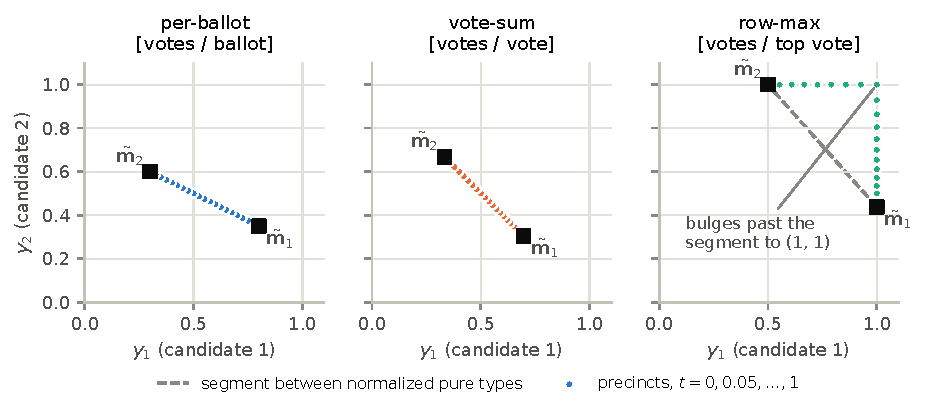
\includegraphics[width=\linewidth]{figures/fig1_geometry.pdf}
  \caption{Two candidates, two voter types, noise-free. Type profiles
  $\m_1=(0.80,0.35)$, $\m_2=(0.30,0.60)$. Their top candidates differ.
  Squares mark the normalized pure types. Dots are precincts with type-2
  fraction $t$.}
  \label{fig:geometry}
\end{figure}

\paragraph{Twelve candidates, three types.} Type 1 votes a wide slate ($c_1=5.6$
names per ballot, top candidate 1). Type 2 is medium ($c_2=3.7$, top candidate 9).
Type 3 is narrow ($c_3=2.25$, top candidate 12). Every other candidate gets
probability $0.05$. Precincts: $n=4000$, $\s_j\sim\mathrm{Dirichlet}(0.7,0.7,0.7)$,
$B_j\sim\mathrm{Unif}\{200,\dots,799\}$. Over these precincts $\Lambda$ has median
$1.48$ and maximum $2.31$.

Figure~\ref{fig:abund} is noise-free and uses the true endmembers $\tilde\M$.
Fitting abundances with SUNSAL (non-negative, sum-to-one) recovers $\Sm$ exactly
under per-ballot. Under vote-sum it recovers the vote-share reweighting of
Proposition~\ref{prop:sum}, again with zero residual. The reweighting depends on
all of $\s_j$ through $\mathbf c^\top\s_j$, hence the band. Under row-max the
residual is not zero: its largest value is $1.48$, and it grows with
$\Lambda-1$. Dropping the ASC brings the residual back to zero
(Corollary~\ref{cor:cone}).

\begin{figure}[ht]
  \centering
  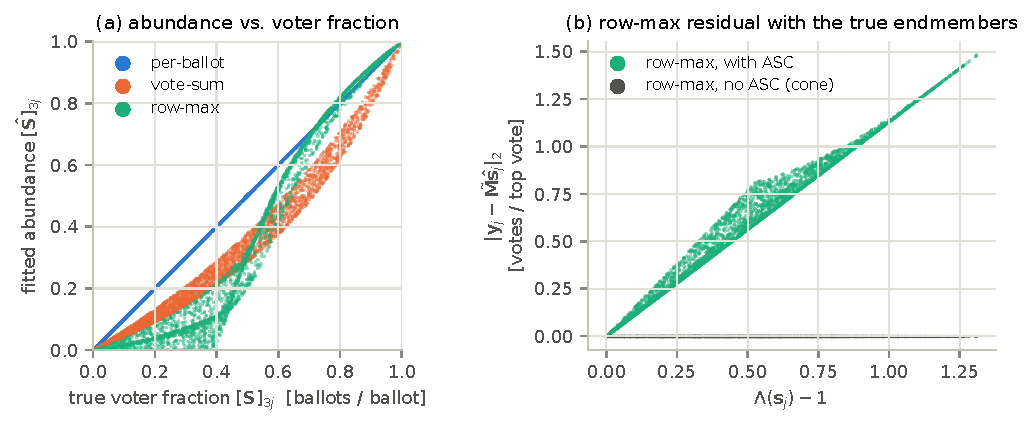
\includegraphics[width=\linewidth]{figures/fig2_abundances.pdf}
  \caption{Noise-free toy election, true endmembers. (a) Fitted abundance of the
  narrow-slate type against its true voter fraction. (b) Row-max residual
  against $\Lambda(\s_j)-1$, with and without the sum-to-one constraint.
  Per-ballot and vote-sum residuals are zero to solver tolerance ($<10^{-6}$)
  and are not shown.}
  \label{fig:abund}
\end{figure}

\paragraph{Blind MVSA on noisy counts (Figure~\ref{fig:mvsa},
Table~\ref{tab:mvsa}).} Counts
$[\mathbf V]_{\ell j}\sim\mathrm{Binomial}(B_j,[\M\s_j]_\ell)$, then each
normalization, then the pipeline's MVSA (\texttt{extract\_endmembers}, $p=3$, best
of 5 seeds by RMSE) and SUNSAL. The ``noise floor'' is the RMSE of the cone fit
with the true endmembers; it is what sampling noise alone costs. Per-ballot
recovers the profiles and their widths, with no negative loadings and RMSE at the
floor. Vote-sum also fits at the floor. Its few small negatives sit where the true
loadings are near zero ($0.05/c_i$) and come from noise. Row-max is $3\times$
the floor even after MVSA picks its own endmembers. It inflates the column sums
by 28--59\% and produces negative loadings down to $-17\%$ of the largest true
loading. The true profiles have no negative loadings, so these come from the
normalization.

\begin{figure}[ht]
  \centering
  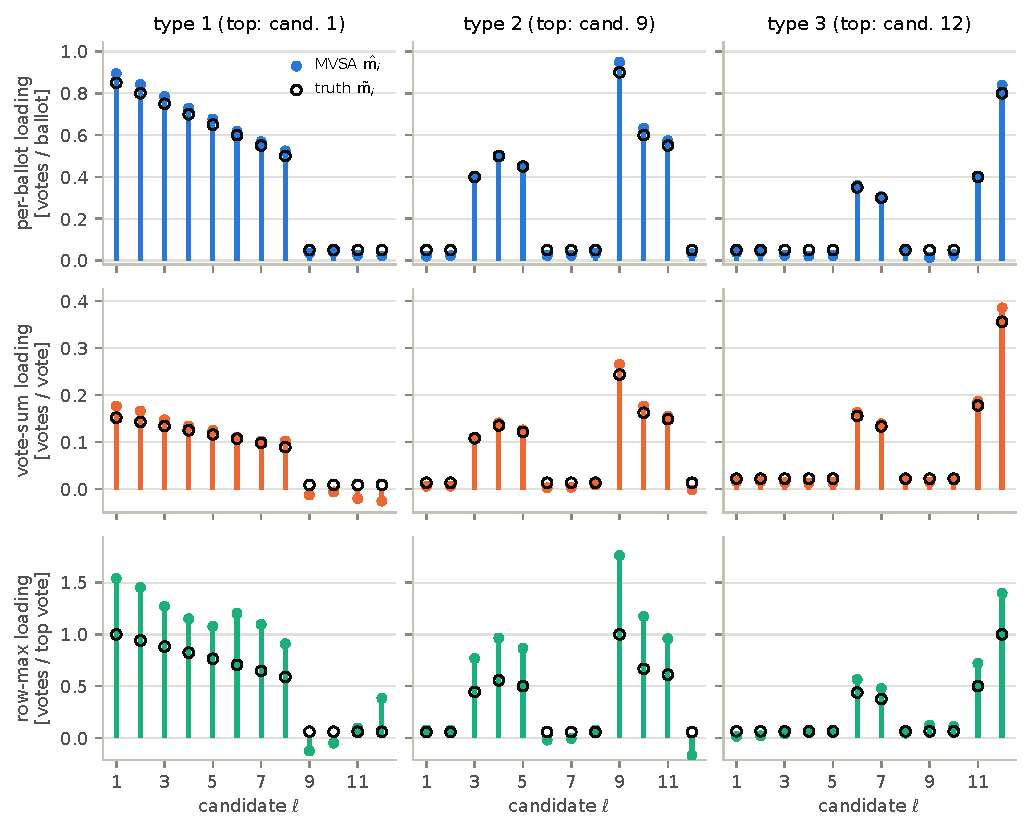
\includegraphics[width=\linewidth]{figures/fig3_mvsa.pdf}
  \caption{Blind MVSA endmembers $\hat\M$ (filled, stems) against the true
  normalized profiles $\tilde\M$ (open circles), matched by cosine. Rows:
  normalization. Columns: voter type. Each row has its own scale.}
  \label{fig:mvsa}
\end{figure}

\begin{table}[ht]
  \centering
  \small
  \resizebox{\linewidth}{!}{\begin{tabular}{lrrrrrll}
\toprule
 & \multicolumn{3}{c}{RMSE $/$ noise floor} & \multicolumn{4}{c}{blind MVSA endmembers $\hat{\mathbf M}$} \\
\cmidrule(lr){2-4}\cmidrule(lr){5-8}
normalization & true $\tilde{\mathbf M}$ & MVSA & noise floor & min loading & \# negative & column sums & true column sums \\
\midrule
per-ballot & 1.05 & 1.05 & 0.0180 & 1.6\% & 0 & 5.76/3.67/2.14 & 5.60/3.70/2.25 \\
vote-sum & 1.00 & 1.00 & 0.0049 & -7.1\% & 4 & 1.00/1.00/1.00 & 1.00/1.00/1.00 \\
row-max & 6.02 & 3.03 & 0.0325 & -16.8\% & 4 & 10.01/6.52/3.61 & 6.59/4.11/2.81 \\
\bottomrule
\end{tabular}
}
  \caption{Noisy toy election, $p=3$. RMSE columns are relative to the noise floor
  (absolute floor in the third column). ``Min loading'' and ``\# negative''
  (loadings below $-1\%$) are relative to the largest true loading, because the
  scales differ by normalization.}
  \label{tab:mvsa}
\end{table}

\section{What this means for the election data}

\begin{enumerate}
  \item Per-ballot normalization is the only one of the three whose abundances
  are voter fractions and whose endmember column sums are names per ballot
  (Proposition~\ref{prop:ballot}). This requires a denominator that counts
  voters. For 2025 that means \texttt{numberOfActuallyVoters}, not
  \texttt{numberOfValidBallot} (Remark~\ref{rem:blank}).
  \item Row-max does not just rescale the per-ballot results. Wherever the mixed
  groups disagree on the top candidate, it moves precincts off the simplex
  (Proposition~\ref{prop:rowmax}), and no set of $p$ endmembers can bring them
  all back (Theorem~\ref{thm:rowmax}). On toy data with no negative loadings at
  all, it produces negative, inflated MVSA endmembers. Some of the 2013/2016
  negative loadings may therefore come from the normalization. The 2019--2025
  mostly-negative archetype cannot be explained this way, because those years
  are per-ballot.
  \item Switching every year to row-max would make the years comparable in
  normalization, but by applying this distortion to all of them. Abundances would
  stop being voter fractions in every year. A cleaner check is to run
  2019--2025 under both per-ballot and row-max. Political change is held fixed
  there, so any difference measures the normalization effect directly.
\end{enumerate}

\paragraph{Reference.} J.~Li and J.~M.~Bioucas-Dias, ``Minimum volume simplex
analysis: a fast algorithm to unmix hyperspectral data,'' in \emph{Proc.\ IEEE
IGARSS}, 2008, vol.~3, pp.~III-250--III-253.

\end{document}
